\documentclass[12pt]{article}

\usepackage{mathrsfs,amsmath}
\usepackage{xcolor}
\usepackage{titlesec}
\usepackage{mwe}
\usepackage{graphicx}
\usepackage{booktabs}
\usepackage{makecell}
\usepackage{array}
\usepackage{float}

\usepackage[margin=1.4in]{geometry}

\title{SRS Documentation| MathGames CS-362}
\author{Jared Dyreson, Peyman Dinani, Kevin Durate \\
        California State University, Fullerton}
\date

\usepackage [english]{babel}
\usepackage [autostyle, english = american]{csquotes}
\MakeOuterQuote{"}


\renewcommand\theadalign{bc}
\renewcommand\theadfont{\bfseries}
\renewcommand\theadgape{\Gape[4pt]}
\renewcommand\cellgape{\Gape[4pt]}


\usepackage{titling}
\renewcommand\maketitlehooka{\null\mbox{}\vfill}
\renewcommand\maketitlehookd{\vfill\null}

\titlespacing*{\section}
{0pt}{5.5ex plus 1ex minus .2ex}{4.3ex plus .2ex}
\titlespacing*{\subsection}
{0pt}{5.5ex plus 1ex minus .2ex}{4.3ex plus .2ex}

\usepackage{hyperref}
\hypersetup{
    colorlinks,
    citecolor=black,
    filecolor=black,
    linkcolor=black,
    urlcolor=blue
}

\graphicspath{ {./assets/} }

\begin{document}

\begin{titlingpage}
\maketitle
\end{titlingpage}

\newpage

\tableofcontents

\newpage

\section{Introduction}

\subsection{Purpose}

The following document contain the software requirements specified for our CPSC362 MathGames game. 
The document will go through the detail, purpose, implementation, and software requirements of MathGames.

\subsection{Scope of the problem}

Learning math can be challenging at times. 
MathGames is designed to take advantage of the internet of things to make practicing math simple, enjoyable and even competitive. 
By utilizing easy to use and seamless networking with other MathGames users, it provides an environment to better engage the math learners. 
MathGames distracts the players of the tedious nature of practicing math by letting players compete against each other in an enjoyable way.    

\subsection{Intended Audience}

MathGames is designed for first graders with simplicity in mind. 
The main focus of MathGames is ease of use and connecting with other MathGames players.

\newpage

\section{Overall Description}

\subsection{User Objectives}

The objective for the end user is to get a better understanding of basic mathematics, mostly intended for children of the ages five to seven.

\subsection{Product Functions}

This product acts as a simple application to answer questions presented by the program to test the child's knowledge.

\subsection{Operating Environment}

\label{marker}

This product has been tested on both Windows and Linux based operating systems.
Intended target for server deployment is Ubuntu server, however other distributions should work out of the box with limited configuration.
For local testing, system administrators can run the project locally and are able to connect to it that way.

The steps for this are as follows:

\begin{itemize}
\item Navigate to the root folder of the MathGames project
\item Open another console window in that current folder
\item Run the following command to instantiate the web server "python Webserver/Server.py"
\item After that, you can run "python main.py" in the other console window, and there should appear an interface asking for login credentials
\end{itemize}

\subsection{Similar System Information}

There are hundreds of other applications that serve the same functionality as MathGames.
However, most of them are single player and do not involve other peers.

\subsection{User Characteristics}

The intended audience does not need any prior technical knowledge and can use this software independently.

\subsection{Design and Implementation Constraints}
The design of this software has led to a simple timing issue between the client machine and the deployed web server. 
Since the Python web server sends information every second, the graphical interface needs to keep up with it. 
That being said, whatever is added in further iterations must keep this dynamic in mind.

\subsection{Assumptions and Dependencies}

\begin{flushleft}

This SRS assumes that:

\begin{itemize}
\item User understands simple English
\item User understands how to do basic arithmetic, such as addition and subtraction
\item An estimate of less than 1 megabyte of disk space is required to install this application
\end{itemize}

List of dependencies include:

\begin{itemize}
\item \href{https://pypi.org/project/websocket_client/}{websocket-client} | an API that interfaces with WebSocket
\item \href{http://pyglet.org/}{pyglet} | an API that allows for the playing of audio cross-platform
\end{itemize}

These dependencies can be installed by running "pip install websocket-client pyglet" and should be handled by the system administrator.
It is not expected for the end user to handle installation of dependencies.

\end{flushleft}

\newpage

\section{Functional Requirements}

\begin{flushleft}

\subsection{The app shall display a login page}

\textbf{Description:} upon clicking the "main.py" file in the root of the project directory, two different windows can appear. If there are no errors with establishing a connection to the server, it will prompt them for their name. Else, it will cease execution and inform the user to enable the server.

\textbf{Pre-condition:} User has downloaded MathGames.

\textbf{Post-condition:} The login screen is displayed.


\subsection{The application shall communicate with the web server}

\textbf{Description:} A connection is established between the client and the server to begin the game

\textbf{Pre-condition:} User has entered the correct information in the login screen

\textbf{Post-condition:} The user will be greeted with the game window

\subsection{The application shall display the game screen}

\textbf{Description:} The game will begin and the user can select input to send to the server

\textbf{Pre-condition:} The game window has appeared to the user

\textbf{Post-condition:} The user can thus begin playing.

\subsection{The application shall play a happy sound and an overlay}

\textbf{Description:} The game will utter a chime that indicates that the user has given the correct input.

\textbf{Pre-condition:} Correct response was given

\textbf{Post-condition:} Chime is played to the user and a small window is shown, displaying a happy face


\subsection{The application shall play a sad sound and an overlay}

\textbf{Description:} The game will utter a sad sound that indicates that the user has given the incorrect input.

\textbf{Pre-condition:} Incorrect response was given.

\textbf{Post-condition:} Sound is played and a small window is shown, displaying a frowning face.

\end{flushleft}

\newpage

\section{Quality Attributes for MathGames}

\begin{table}[H]
\begin{tabular}{@{}|l|l|@{}}
\toprule
\textbf{Quality Attribute} & \textbf{Brief Description} \\ \midrule
RT-1 & \makecell{The game will respond to server availability based \\ on the quality of internet connection.} \\ \midrule
RT-1 & \makecell{The game will show an error/ notify user if the server is not \\ available within seconds of launching.} \\ \midrule
SS-1 & \makecell{The game will ask the player name right after \\ launching and checking for server availability.} \\ \midrule
SA-1 & The game will be available as long as the server is up and running. \\ \midrule
AC-1 & \makecell{The game will be accessible by windows or mac computers with \\ python installed and internet connectivity}. \\ \bottomrule
\end{tabular}
\end{table}

\begin{itemize}

\item \textbf{RE: Response Time}
\item \textbf{SS: System Security}
\item \textbf{SA: System Availability}
\item \textbf{AC: System Accessibly}

\end{itemize}

\newpage

\section{Non-Functional Requirements}

\subsection{Security}

There are no current security threats in the latest build of MathGames.

\subsection{Usability}

\begin{itemize}
\item The user will require a working internet connection
\item After starting the application, the user will be required to enter their name in a small text field
\end{itemize}

\subsection{Backup}

\begin{itemize}
\item The latest score of the user will be saved on the server as long as the server has not been reset
\end{itemize}

\newpage

\section{Interface Requirement}

\subsection{GUI}

\subsection{Hardware Interface}

This application is expected to be used on a desktop computer that has an Ethernet connection.
Optionally, you can run this on a laptop with a wireless connection, neither option will degrade the experience of MathGames.

\subsection{Software Interface}

Please refer to the Operating Environment section here \underline{\nameref{marker}}

\newpage

\section{SWOT Analysis for MathGames}

\subsection{Strengths}

\begin{itemize}
\item S1: The application has very little load on the CPU, allowing many lower-powered devices to run this application with minimal resources.
\item S2: The application features eye catching graphics that are intended for younger generations.
\item S3: The application has a minimalistic interface, which is simple for the user to memorize and use.
\end{itemize}

\subsection{Weaknesses}

\begin{itemize}
\item W1: The application asks questions that result in answers from 0 to 10 which may become an issue when the user becomes proficient enough for more advanced mathematics.
\item W2: The application requires the server to be running as it is intended to be a multiplayer game.
\item W3: The application does not pair users based on their skill set. Thus, a new player can possibly be playing against a very experienced player - causing an unfair game.
\end{itemize}

\subsection{Opportunities}

\begin{itemize}
\item O1: This application serves the purpose of providing a quick and intuitive way for younger audiences to practice simple arithmetic. Many other mathematics applications have complex settings, goals, and gameplay mechanics. This program does what it is intended to do and nothing more. This will attract many users as they know exactly what the application is for.
\item O2: This application offers a quick way to play math games in seconds after installing. No need to configure settings or fiddle around with creating an account, just launch the application and type in your name. Many other mathematical applications require account sign ups, long setup process, and more. Parents and guardians can get their child playing almost immediately after installing. 
\item O3: This application does not store any sensitive data nor allow for communication with other players. With the growing fear of software collecting data, parents and guardians often worry what data is being collected on their child. This application keeps parents and guardians at ease since there is no sensitive data collected. 
\end{itemize}

\subsection{Threats}

\begin{itemize}
\item T1: There is no profit to be made from this application as it is free to play without in-app purchases. Thus, sustaining this application will require our company to gather volunteers or pay developers (at a loss) to continually maintain and update it. This is a threat as our company will continually lose money on the application.
\item T2: The audience for this application is very limited as it is intended for very young students. Once a student advances in school, they will most likely not use the application again. This will make it very difficult to achieve long-term users. This is a threat as long-term users help our company grow. If we cannot sustain a strong fan-base, it will be very difficult to expand our company.  
\item T3: The application is not available for mobile devices, which is a problem since younger audiences use mobile devices more than personal computers. As phones become more ubiquitous than personal computers, the less market share we are able to obtain. 
\end{itemize}

\section{UML Diagrams}

\subsection{Use Case Diagram}

\subsection{Sequence Diagram}

\fbox{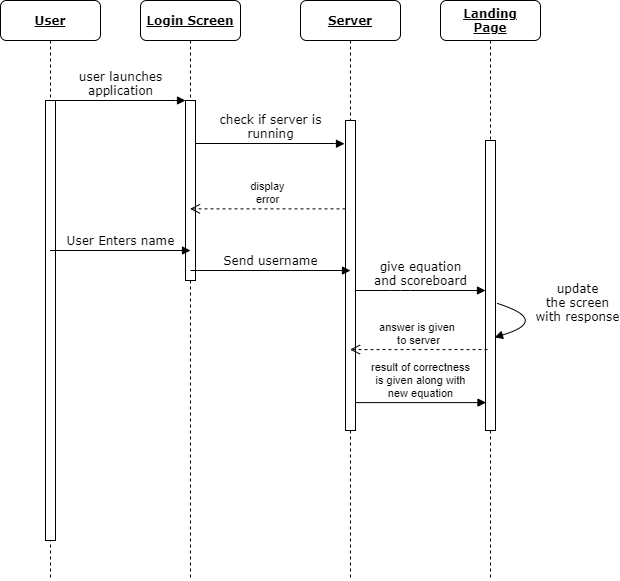
\includegraphics[width=11cm]{SequenceDiagram2.png}}

\subsection{Activity Diagram}

\newpage

\section{References}

\begin{itemize}
\item \href{https://app.diagrams.net/}{Draw.io} | feature rich site to create the UML diagrams in this document
\item \href{https://www.latex-project.org/}{\LaTeX} | powerful typesetting language to create this document
\item \href{https://stackoverflow.com/}{StackOverflow} | for general questions regarding specific areas of interest and program behavior
\end{itemize}

\end{document}
